\chapter{氨基酸与蛋白质}\label{ch:b1:proteins}

煮一个鸡蛋，透明的蛋清会变得不透明、结实；
没有添加或去除任何东西，但其中每个\omterm{def:b1:proteins:peptide}{蛋白质}分子都已展开，
并与邻近分子相互缠结。冷却后它仍保持煮熟的状态。然而，一种小酶
在试管中被温和展开后，置于普通\omterm{def:b1:water-small-molecules:buffer}{缓冲液}中，
数分钟内便重新折叠成精确的工作构象，无需任何外力帮助：
这一形状早已写在肽链之中。\omterm{def:b1:proteins:peptide}{蛋白质}是\omterm{def:b1:cell-unit-of-life:cell}{细胞}的工作分子——
包括它的酶、泵、马达和支架，
抗体和激素——它们每一种都是由\omterm{def:b1:proteins:aminoacid}{氨基酸}组成的链，
并折叠成由其序列决定的形状。本章
介绍二十种\omterm{def:b1:proteins:aminoacid}{氨基酸}、连接它们的\omterm{def:b1:proteins:peptide}{肽键}、\omterm{def:b1:proteins:peptide}{蛋白质}结构的
四个层次、使肽链折叠为机器的过程、
多亚基\omterm{def:b1:proteins:peptide}{蛋白质}的协同行为，
以及分离和观察\omterm{def:b1:proteins:peptide}{蛋白质}的方法。

\section{氨基酸}

\begin{definition}[氨基酸]\label{def:b1:proteins:aminoacid}
\emph{氨基酸}\index{氨基酸}分子有一个中心\emph{$\alpha$ 
碳}连有氨基（$-\mathrm{NH_2}$）、羧基（$-\mathrm{COOH}$），
一个氢和一个\emph{侧链}\index{侧链}
$R$，它使\omterm{def:b1:proteins:peptide}{蛋白质}中的二十种标准氨基酸彼此区别。
在\omterm{def:b1:cell-unit-of-life:cell}{细胞}的 \omterm{def:b1:water-small-molecules:ph}{pH} 下，氨基质子化，羧基
发生电离，分子为\emph{两性离子}\index{两性离子}，
$\mathrm{^+H_3N{-}CHR{-}COO^-}$，净电荷为零。$\alpha$ 碳
除甘氨酸外均为手性，生物只使用 L 型对映异构体。
按化学性质，侧链可分为以下几类：
\begin{center}
\footnotesize
\begin{tabular}{lll}
\hline
类别 & 氨基酸（三字母和单字母代码） & 侧链 \\
\hline
非极性\omterm{def:b1:lipids:triglyceride}{脂肪}族 & Gly G、Ala A、Val V、Leu L、Ile I、Met M、Pro P & 烃基；Pro 为环 \\
芳香族 & Phe F、Tyr Y、Trp W & 芳环；Tyr 和 Trp 吸收紫外光 \\
极性不带电 & Ser S、Thr T、Cys C、Asn N、Gln Q & $-$OH、$-$SH、酰胺 \\
带正电 & Lys K、Arg R、His H & 碱性基团；His 的 p$K_a$ 为 6.0 \\
带负电 & Asp D、Glu E & 羧酸根，p$K_a$ 为 4 \\
\hline
\end{tabular}
\end{center}
其中九种（His、Ile、Leu、Lys、Met、Phe、Thr、Trp、Val）对人类而言是
\emph{必需}的，即人体无法自行合成，必须从食物中摄入。
\end{definition}

\begin{proposition}[电离]\label{prop:b1:proteins:ionisation}
\omterm{def:b1:proteins:aminoacid}{氨基酸}的每个可电离基团都有各自的 p$K_a$：$\alpha$-羧基约为 2，
$\alpha$-氨基约为 9.5，\omterm{def:b1:proteins:aminoacid}{侧链}则分别为
3.9（Asp）、4.1（Glu）、6.0（His）、8.3（Cys）、10.1（Tyr）、10.5
（Lys）、12.5（Arg）。\emph{等电点}\index{等电点} p$I$ 是净电荷为零时的 \omterm{def:b1:water-small-molecules:ph}{pH}——
即夹住中性形式的两个 p$K_a$ 的平均值；\omterm{def:b1:proteins:peptide}{蛋白质}的 p$I$ 由
其带电\omterm{def:b1:proteins:aminoacid}{侧链}的含量决定，此时溶解度最低，
且在电场中不发生迁移。组氨酸的 p$K_a$
接近 7，是在生理范围内改变电荷的残基，
并常位于许多酶的活性位点中。
\end{proposition}

\begin{omfigure}
\begin{tikzpicture}
\begin{axis}[
  width=0.86\linewidth, height=6.0cm,
  axis x line=bottom, axis y line=left,
  xmin=0, xmax=2.1, ymin=0, ymax=13,
  xlabel={加入的 $\mathrm{OH^-}$ 当量数}, ylabel={pH},
  xlabel style={font=\small, at={(axis description cs:0.5,-0.12)}, anchor=north},
  ylabel style={font=\small},
  tick label style={font=\small}, xtick={0,0.5,1,1.5,2}, ytick={0,2,4,6,8,10,12},
  clip=false,
]
\addplot[very thick, omDef, domain=0.02:0.98, samples=80] {2.34 + log10(x/(1-x))};
\addplot[very thick, omDef, domain=1.02:1.98, samples=80] {9.6 + log10((x-1)/(2-x))};
\addplot[very thick, omDef, domain=0.98:1.02, samples=10] {5.97 + (x-1)*250};
\draw[dashed, gray] (axis cs:0,2.34) -- (axis cs:0.5,2.34); \node[font=\scriptsize, anchor=west] at (axis cs:0.02,3.4) {p$K_1 = 2.34$: $\mathrm{COOH}/\mathrm{COO^-}$};
\draw[dashed, gray] (axis cs:0,9.6) -- (axis cs:1.5,9.6); \node[font=\scriptsize, anchor=north west] at (axis cs:1.52,9.3) {p$K_2 = 9.6$: $\mathrm{NH_3^+}/\mathrm{NH_2}$};
\draw[dashed, gray] (axis cs:0,5.97) -- (axis cs:1,5.97); \node[font=\scriptsize, anchor=south east] at (axis cs:0.98,6.1) {p$I = 5.97$：两性离子};
\node[font=\scriptsize, anchor=west] at (axis cs:0.42,0.9) {$\mathrm{^+H_3N{-}CH_2{-}COOH}$};
\node[font=\scriptsize, anchor=east] at (axis cs:0.93,8.5) {$\mathrm{^+H_3N{-}CH_2{-}COO^-}$};
\node[font=\scriptsize, anchor=south] at (axis cs:1.75,12.0) {$\mathrm{H_2N{-}CH_2{-}COO^-}$};
\end{axis}
\end{tikzpicture}

{\small 甘氨酸的滴定。两个缓冲平台分别对应羧基和氨基的 p$K_a$，
二者之间即\omterm{prop:b1:proteins:ionisation}{等电点}，
此时\omterm{def:b1:proteins:aminoacid}{两性离子}不带净电荷。}
\end{omfigure}

\section{肽键}

\begin{definition}[肽键、多肽]\label{def:b1:proteins:peptide}
\emph{肽键}\index{肽键}通过\omterm{prop:b1:water-small-molecules:families}{缩合}反应，将一个\omterm{def:b1:proteins:aminoacid}{氨基酸}的羧基
与下一个\omterm{def:b1:proteins:aminoacid}{氨基酸}的氨基相连（酰胺键，
$\mathrm{-CO{-}NH-}$）。这样连接的\omterm{def:b1:proteins:aminoacid}{氨基酸}链称为
\emph{多肽}\index{多肽}：其\emph{骨架}由重复的
$\mathrm{N{-}C_\alpha{-}C}$ 单元构成，\omterm{def:b1:proteins:aminoacid}{侧链}由此伸出，
并具有\emph{N 端}（游离氨基）和\emph{C 端}
（游离羧基）。序列按从 N 端到 C 端书写，即合成的顺序
（见\cref{ch:b1:gene-expression}）。\emph{蛋白质}\index{蛋白质}
是由一条或多条多肽折叠成确定形状的分子；典型
肽链含 \qtyrange{100}{1000}{} 个残基，每个残基的平均质量为 \qty{110}{Da}，
因此含 \qty{300}{} 个残基的蛋白质质量为 \qty{33}{kDa}。
\end{definition}

\begin{proposition}[肽键的几何构型]\label{prop:b1:proteins:geometry}
\omterm{def:b1:proteins:peptide}{肽键}中的 C--N 键具有部分双键性质（
即酰胺共振）：该键很短，不能旋转，并使六个原子
$\mathrm{C_\alpha{-}C(=O){-}N(H){-}C_\alpha}$ 位于同一平面内，几乎总是
两个 $\alpha$ 碳呈\emph{反式}。骨架因此是
由刚性平面构成的链，各平面以 $\alpha$ 碳为铰链连接，每个
铰链有两种旋转：$\phi$（绕 N--$\mathrm{C_\alpha}$ 键）和
$\psi$（绕 $\mathrm{C_\alpha}$--C 键）；\omterm{def:b1:proteins:aminoacid}{侧链}与骨架之间的空间冲突
禁止了 $\phi$ 与 $\psi$ 的大多数组合。
\omterm{def:b1:proteins:peptide}{蛋白质}的构象本质上就是其全部的 $\phi$ 与
$\psi$ 角的列表。
\end{proposition}

\begin{omfigure}
\begin{tikzpicture}[font=\footnotesize, line cap=round]
  % two peptide planes
  \fill[omDef!12, rounded corners=3pt] (0.3,-0.9) rectangle (3.3,0.9);
  \fill[omDef!12, rounded corners=3pt] (3.9,-0.9) rectangle (6.9,0.9);
  % atoms
  \node (ca1) at (0,0) {$\mathrm{C_\alpha}$};
  \node (c1) at (1.2,0.4) {C};
  \node (o1) at (1.2,1.3) {O};
  \node (n1) at (2.4,-0.4) {N};
  \node (h1) at (2.4,-1.3) {H};
  \node (ca2) at (3.6,0) {$\mathrm{C_\alpha}$};
  \node (c2) at (4.8,0.4) {C};
  \node (o2) at (4.8,1.3) {O};
  \node (n2) at (6.0,-0.4) {N};
  \node (h2) at (6.0,-1.3) {H};
  \node (ca3) at (7.2,0) {$\mathrm{C_\alpha}$};
  \draw[thick] (ca1) -- (c1); \draw[thick, double] (c1) -- (o1); \draw[very thick, omThm] (c1) -- (n1); \draw[thick] (n1) -- (h1); \draw[thick] (n1) -- (ca2);
  \draw[thick] (ca2) -- (c2); \draw[thick, double] (c2) -- (o2); \draw[very thick, omThm] (c2) -- (n2); \draw[thick] (n2) -- (h2); \draw[thick] (n2) -- (ca3);
  % side chains
  \draw[thick] (ca1) -- ++(-0.5,-0.8) node[below] {$R_1$};
  \draw[thick] (ca2) -- ++(0,-1.0) node[below] {$R_2$};
  \draw[thick] (ca3) -- ++(0.5,-0.8) node[below] {$R_3$};
  % rotation arrows phi/psi at ca2
  \draw[->, omProp, thick] (2.9,-0.55) arc (200:340:0.35); \node[omProp, font=\scriptsize] at (3.05,-0.95) {$\phi$};
  \draw[->, omProp, thick] (3.85,0.55) arc (160:20:0.35); \node[omProp, font=\scriptsize] at (4.2,1.0) {$\psi$};
  \node[anchor=west, align=left] at (7.9,0.6) {\textcolor{omThm}{红色}：肽键，平面，\\ 不能旋转（部分双键）};
  \node[anchor=west, align=left] at (7.9,-0.5) {\textcolor{omProp}{橙色}：两个自由旋转 \\ $\phi$ 与 $\psi$，位于每个 $\alpha$ 碳处};
\end{tikzpicture}

{\small 两个\omterm{def:b1:proteins:peptide}{肽键}。每个阴影平面刚性地包含六个原子；
肽链仅在 $\alpha$ 碳处弯折，弯折角为 $\phi$
与 $\psi$。}
\end{omfigure}

\section{二级结构}

\begin{definition}[二级结构]\label{def:b1:proteins:secondary}
\omterm{def:b1:proteins:peptide}{蛋白质}的\emph{二级结构}\index{二级结构}
是指其骨架的局部规则折叠，由\omterm{def:b1:water-small-molecules:water}{氢键}维持，
\omterm{def:b1:water-small-molecules:water}{氢键}位于骨架 C=O 与 N--H 基团之间。主要有两种模式。
\emph{$\alpha$ 螺旋}\index{alpha helix@$\alpha$ 螺旋}：右手螺旋，
每圈 3.6 个残基，每个残基上升 \qty{0.15}{nm}
（每圈 \qty{0.54}{nm}），每个 C=O 与前方第四个残基的 N--H 形成\omterm{def:b1:water-small-molecules:water}{氢键}，
\omterm{def:b1:proteins:aminoacid}{侧链}指向外侧。\emph{$\beta$
折叠}\index{beta sheet@$\beta$ 折叠}：肽链几乎完全伸展
（每个残基 \qty{0.35}{nm}），并排排列，可平行或
反平行，相邻链之间由\omterm{def:b1:water-small-molecules:water}{氢键}相连，\omterm{def:b1:proteins:aminoacid}{侧链}
在折叠面上下交替排列。两者之间，\emph{转角}和
环区使肽链走向反转。脯氨酸的环状结构锁定了 $\phi$，
因而破坏螺旋；甘氨酸没有\omterm{def:b1:proteins:aminoacid}{侧链}，允许形成其他残基都无法形成的
转角。
\end{definition}

\begin{omfigure}
\begin{tikzpicture}
\begin{axis}[
  width=0.62\linewidth, height=6.4cm,
  axis x line=bottom, axis y line=left,
  xmin=-180, xmax=180, ymin=-180, ymax=180,
  xlabel={$\phi$（度）}, ylabel={$\psi$（度）},
  xlabel style={font=\small, at={(axis description cs:0.5,-0.12)}, anchor=north},
  ylabel style={font=\small},
  tick label style={font=\small}, xtick={-180,-90,0,90,180}, ytick={-180,-90,0,90,180},
  clip=false,
]
\fill[omDef!35] (axis cs:-160,90) rectangle (axis cs:-50,180);
\fill[omDef!35] (axis cs:-160,-180) rectangle (axis cs:-50,-150);
\fill[omThm!35] (axis cs:-150,-70) rectangle (axis cs:-45,-10);
\fill[omExo!35] (axis cs:40,10) rectangle (axis cs:80,70);
\node[font=\scriptsize] at (axis cs:-105,140) {$\beta$ 折叠};
\node[font=\scriptsize] at (axis cs:-97,-40) {右手 $\alpha$ 螺旋};
\node[font=\scriptsize, align=center] at (axis cs:60,100) {左手螺旋 \\ （仅甘氨酸）};
\node[font=\scriptsize, gray, align=center] at (axis cs:80,-100) {白色：因 \\ 空间冲突而禁止};
\draw[gray] (axis cs:-180,0) -- (axis cs:180,0); \draw[gray] (axis cs:0,-180) -- (axis cs:0,180);
\end{axis}
\end{tikzpicture}

{\small 拉马钱德兰图：残基所能采取的 $\phi$ 与 $\psi$ 组合。
两个较大的允许区域分别对应
$\beta$ 折叠和右手 $\alpha$ 螺旋；图中大部分
区域因原子间碰撞而被禁止。}
\end{omfigure}

\begin{omfigure}
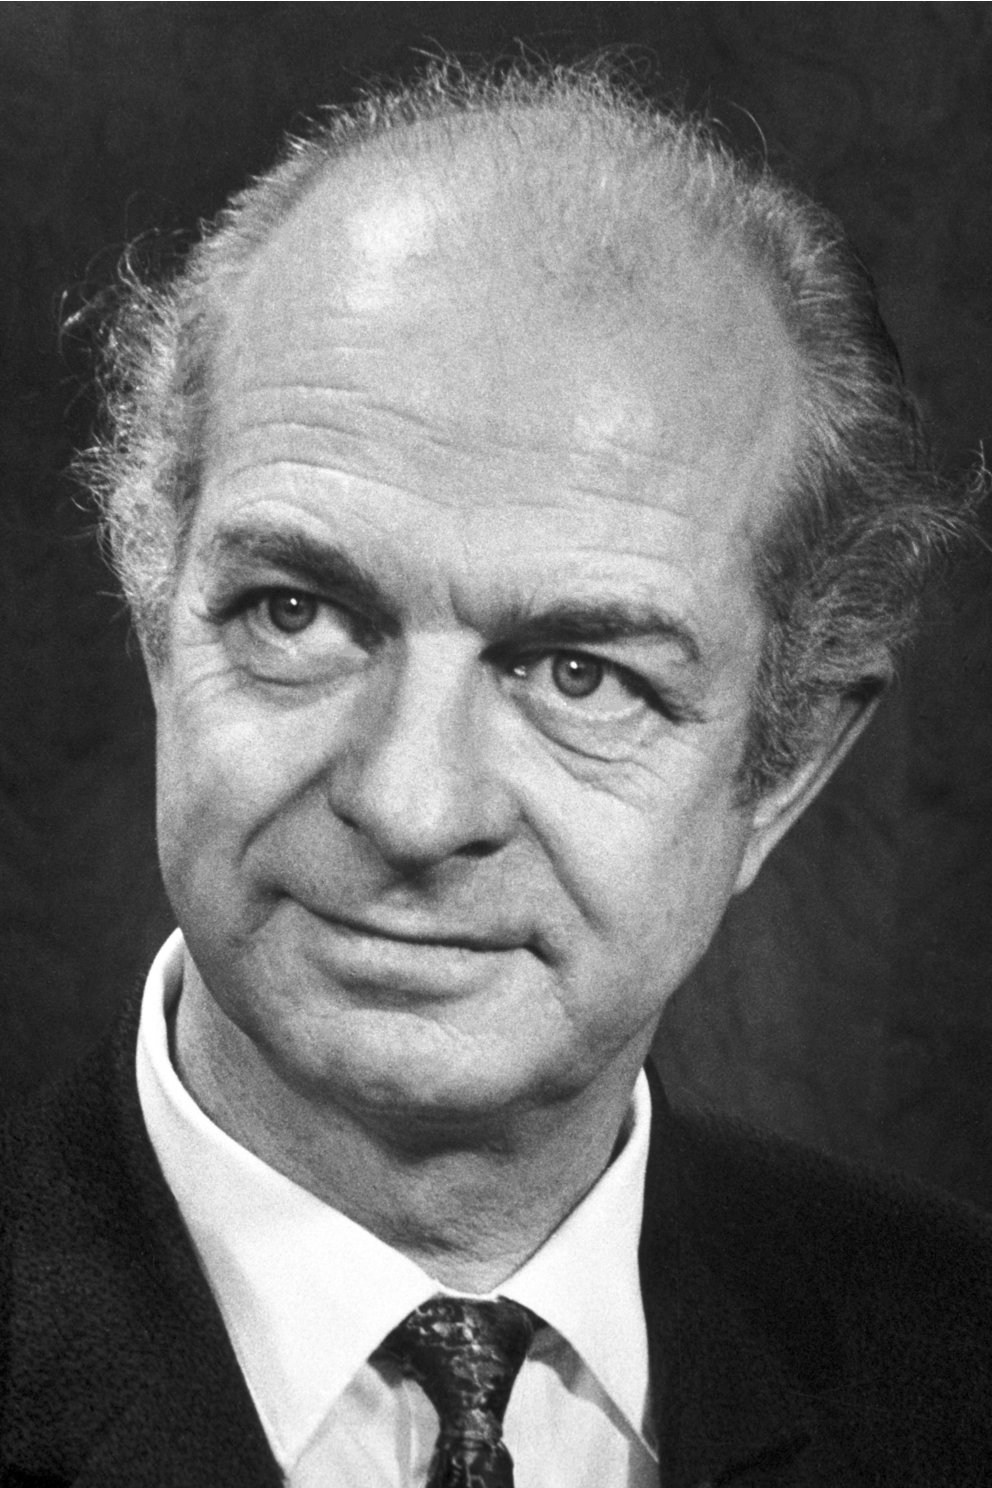
\includegraphics[width=0.26\linewidth]{images/book3/pauling.jpg}

{\small 莱纳斯·鲍林（1901--1994），他于 1951 年推导出 $\alpha$ 螺旋和
$\beta$ 折叠，依据是\omterm{def:b1:proteins:peptide}{肽键}的平面性与\omterm{def:b1:water-small-molecules:water}{氢键}的几何构型，
而当时这两种结构都尚未在\omterm{def:b1:proteins:peptide}{蛋白质}中被观察到。
照片：Nobel Foundation，1962，公有领域。}
\end{omfigure}

\begin{example}[用数字看螺旋与折叠]\label{ex:b1:proteins:numbers}
跨膜 $\alpha$ 螺旋必须穿过 \qty{3}{nm} 的
疏水核心：$3/0.15 = 20$ 个残基，而且在
\cref{ch:b1:membranes-transport}中的跨膜片段确实是
约二十个疏水残基组成的连续段。长度相同的 $\beta$ 链跨度为
\qty{7}{nm}：丝心蛋白是由甘氨酸和丙氨酸组成的反平行折叠片层堆叠而成，
丝线比同等重量的钢更坚韧，
是因为共价骨架沿纤维方向排列。
\end{example}

\section{三级与四级结构}

\begin{definition}[三级结构与四级结构]\label{def:b1:proteins:tertiary}
\emph{三级结构}\index{三级结构}是指单条\omterm{def:b1:proteins:peptide}{多肽}链完整的
三维空间排布，即其螺旋、折叠
和环区紧密\omterm{prop:b1:nucleic-acids:stability}{堆积}在一起，常形成若干可独立折叠的紧凑\emph{结构域}。
它由非共价作用维持——
\emph{\omterm{prop:b1:water-small-molecules:properties}{疏水效应}}使非极性\omterm{def:b1:proteins:aminoacid}{侧链}埋在远离水的核心中，
此外还有\omterm{def:b1:water-small-molecules:water}{氢键}、带电\omterm{def:b1:proteins:aminoacid}{侧链}之间的盐桥以及
\omterm{def:b1:water-small-molecules:bonds}{范德华}\omterm{prop:b1:nucleic-acids:stability}{堆积}——有时还由\emph{二硫键}
\index{二硫键}维持，即两个半胱氨酸之间共价的 S--S 键，
见于分泌到氧化性胞外\omterm{def:b1:organism-environment:organism}{环境}中的\omterm{def:b1:proteins:peptide}{蛋白质}。
\emph{四级结构}\index{四级结构}是指若干条\omterm{def:b1:proteins:peptide}{多肽}链
（亚基）组装成一个\omterm{def:b1:proteins:peptide}{蛋白质}：
血红蛋白由两条 $\alpha$ 链和两条 $\beta$ 链组成。\emph{球状}
\omterm{def:b1:proteins:peptide}{蛋白质}紧凑且可溶于水（如酶、\omterm{def:b1:membranes-transport:transporters}{载体蛋白}）；
\emph{纤维状}\omterm{def:b1:proteins:peptide}{蛋白质}伸展且不溶（如\omterm{def:b1:body-plans-tissues:connective}{胶原蛋白}的三螺旋、
角蛋白和肌球蛋白的卷曲螺旋，以及丝蛋白）。
\end{definition}

\begin{omfigure}
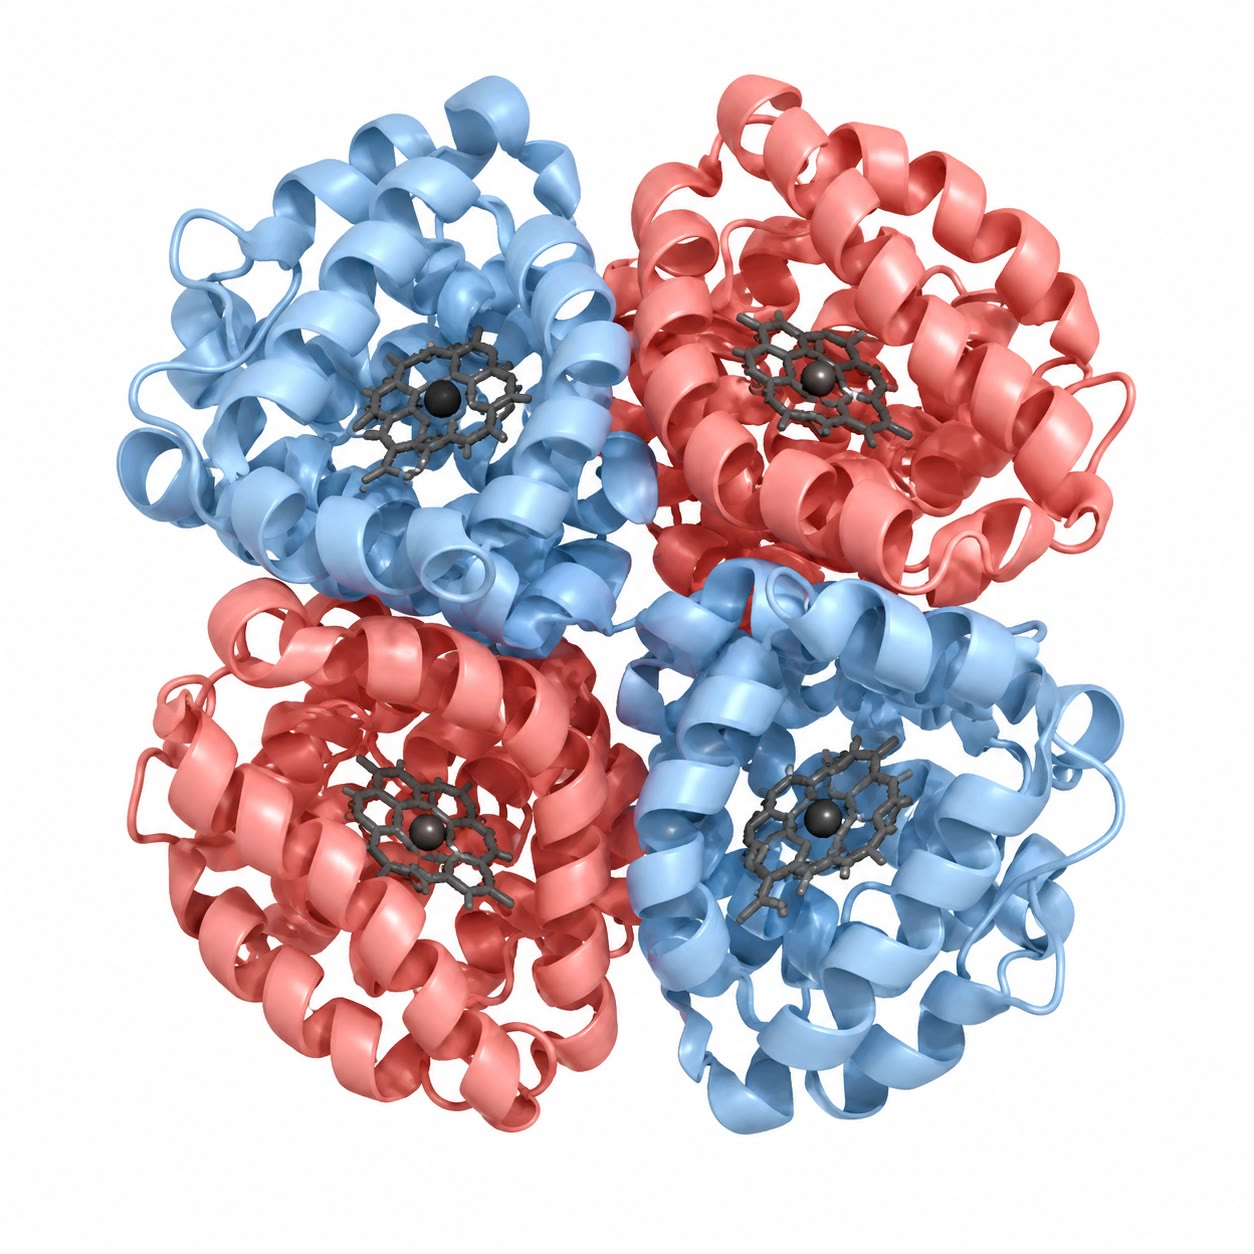
\includegraphics[width=0.42\linewidth]{images/book3/ai/fig-hemoglobin-ribbon.jpg}

{\small 血红蛋白：四个亚基，两条 $\alpha$ 链（蓝色）和两条 $\beta$ 链
（红色），每条都是围绕血红素基团（深色）的 $\alpha$ 螺旋束，
其铁原子结合一个 $\mathrm{O_2}$。四个结合位点并非
彼此独立地起作用。}
\end{omfigure}

\begin{theorem}[序列决定折叠方式]\label{thm:b1:proteins:anfinsen}
\index{蛋白质折叠}
\omterm{def:b1:proteins:peptide}{蛋白质}的三维结构由其\omterm{def:b1:proteins:aminoacid}{氨基酸}序列决定：天然折叠态
是\omterm{def:b1:proteins:peptide}{多肽}链在\omterm{def:b1:cell-unit-of-life:cell}{细胞}\omterm{def:b1:organism-environment:organism}{环境}中能够达到的\omterm{prop:b1:water-small-molecules:gibbs}{自由能}最低的构象，
而达到该构象所需的信息
就包含在\omterm{def:b1:proteins:peptide}{多肽}链本身之中。
\end{theorem}
\begin{proof}[证据]
安芬森（1961 年）将核糖核酸酶 A 展开，该酶含 \qty{124}{} 个残基，
带有四个\omterm{def:b1:proteins:tertiary}{二硫键}。他将其置于浓尿素中，
并加入可断开\omterm{def:b1:proteins:tertiary}{二硫键}的还原剂，\omterm{def:b1:proteins:peptide}{多肽}链随即失去全部活性。
去除尿素后，让半胱氨酸在空气中缓慢再氧化，
他使酶完全恢复活性，四个\omterm{def:b1:proteins:tertiary}{二硫键}在同样的八个半胱氨酸之间重新形成，
在 \qty{105}{} 种可能的配对中。
\omterm{def:b1:proteins:peptide}{多肽}链找到了它自己的折叠方式。若在尿素中即行再氧化，
则形成随机的\omterm{def:b1:proteins:tertiary}{二硫键}，酶保持无活性；随后加入少量还原剂，
使\omterm{def:b1:proteins:tertiary}{二硫键}不断重排，直至达到最稳定的天然组合。
此后，人们已在试管中从头折叠了数千种
序列，
并可由新序列计算出其折叠结构。
\end{proof}

\begin{proposition}[变性]\label{prop:b1:proteins:denaturation}
\index{变性（蛋白质）}
加热、极端 \omterm{def:b1:water-small-molecules:ph}{pH}、尿素、去污剂或有机溶剂，会压倒维持折叠的弱键，
从而使\omterm{def:b1:proteins:peptide}{蛋白质}展开：\omterm{def:b1:proteins:peptide}{多肽}链失去其形状和功能，
暴露其疏水核心，并与邻近分子聚集在一起。
小分子\omterm{def:b1:proteins:peptide}{蛋白质}在去除\omterm{def:b1:nucleic-acids:melting}{变性}剂后可以重新折叠；
大分子\omterm{def:b1:proteins:peptide}{蛋白质}，以及拥挤\omterm{def:b1:cell-unit-of-life:cell}{细胞}中的\omterm{def:b1:proteins:peptide}{蛋白质}，往往无法复性，
于是\omterm{def:b1:cell-unit-of-life:cell}{细胞}保留\emph{分子伴侣}\index{分子伴侣}——
它们结合未折叠的\omterm{def:b1:proteins:peptide}{多肽}链，遮蔽其疏水表面，
并多次给予其正确折叠的机会——并降解仍然错误折叠的部分。
发热数度，以及脑蛋白开始展开的 \qty{42}{\celsius}，
标志着稳定性的狭窄余量：
典型的折叠结构仅比未折叠的\omterm{def:b1:proteins:peptide}{多肽}链稳定 \qtyrange{20}{60}{kJ/mol}，
相当于几个\omterm{def:b1:water-small-molecules:water}{氢键}的强度。
\end{proposition}

\begin{omfigure}
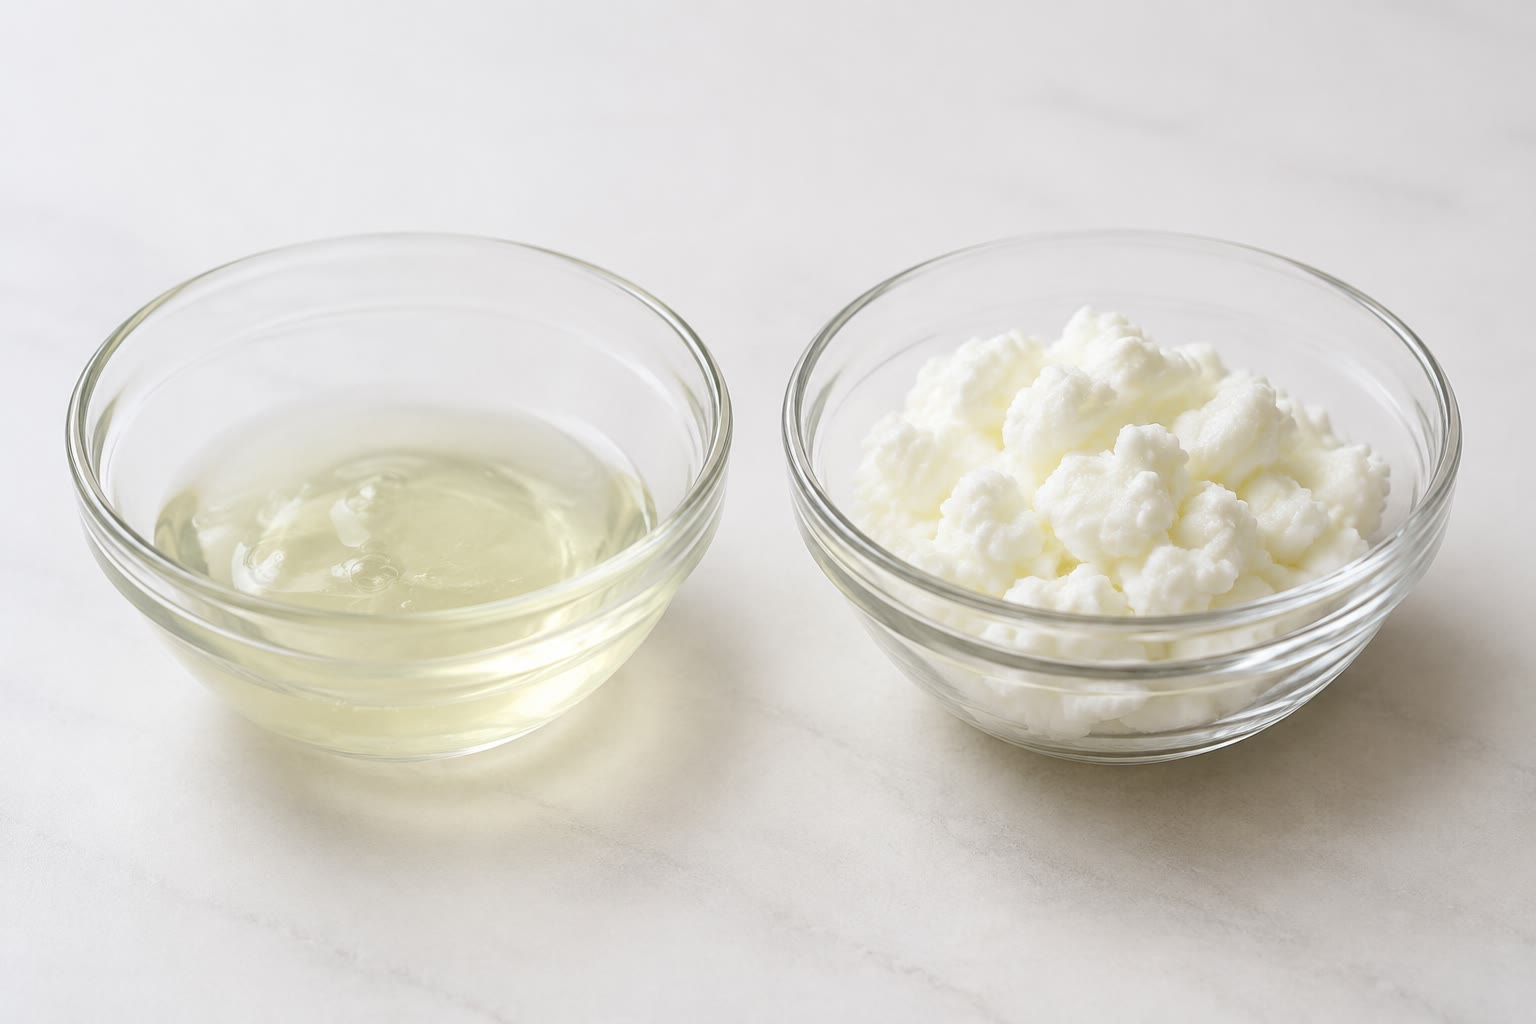
\includegraphics[width=0.5\linewidth]{images/book3/ai/b3-12-egg-white-cooked.jpg}

{\small 生鸡蛋清与煮熟的蛋清：同样的\omterm{def:b1:proteins:peptide}{蛋白质}，左侧为折叠且可溶的状态，
右侧展开并聚集成不透明的固体。
除加热外，未添加任何物质。}
\end{omfigure}

\begin{example}[胶原蛋白]\label{ex:b1:proteins:collagen}
哺乳动物\omterm{def:b1:proteins:peptide}{蛋白质}的四分之一是\omterm{def:b1:body-plans-tissues:connective}{胶原蛋白}：三条链，每条都是由一千个残基组成的左手螺旋，
每隔两个残基（即第三位）为甘氨酸（Gly--X--Y，Y 常为羟脯氨酸），
三条链缠绕成右手三螺旋，长 \qty{300}{nm}，
再并排\omterm{prop:b1:nucleic-acids:stability}{堆积}成由\omterm{def:b1:water-small-molecules:bonds}{共价键}交联的原纤维。
甘氨酸没有\omterm{def:b1:proteins:aminoacid}{侧链}，因此三条链才能
在中轴处紧密\omterm{prop:b1:nucleic-acids:stability}{堆积}；若将甘氨酸替换为任何其他残基，螺旋便会弯折，导致\omterm{def:b1:body-plans-tissues:segments}{骨骼}脆弱。
维生素 C 是羟化脯氨酸所必需的；
缺乏它，螺旋便不稳定，原纤维失效：
即坏血病。
\end{example}

\section{别构作用：血红蛋白}

\begin{definition}[别构作用，协同性]\label{def:b1:proteins:allostery}
当配体在某一位点的结合改变了\omterm{def:b1:proteins:peptide}{蛋白质}的构象，从而改变其在另一位点的亲和力时，
该\omterm{def:b1:proteins:peptide}{蛋白质}称为\emph{别构的}\index{别构作用}。
若各位点相同，且这一改变提高了其他位点的亲和力，
则称结合具有\emph{协同性}\index{协同性}：
饱和曲线呈 S 形而非双曲线形，
\omterm{def:b1:proteins:peptide}{蛋白质}在较窄的配体浓度范围内由几乎全空迅速变为几乎全满。
\emph{希尔方程}\index{希尔方程}
描述了这一过程：
\[
Y = \frac{P^n}{P_{50}^n + P^n},
\]
其中 $Y$ 为被占据位点的比例，$P$ 为配体
浓度（或分压），$P_{50}$ 为半饱和时的值，
$n$ 为希尔系数——位点独立时为 1，
完全协同时可达位点的总数。
\end{definition}

\begin{proposition}[血红蛋白与肌红蛋白]\label{prop:b1:proteins:hemoglobin}
肌红蛋白是只含一条链和一个血红素的\omterm{def:b1:proteins:peptide}{蛋白质}，
其结合 $\mathrm{O_2}$ 的曲线为双曲线（$n = 1$，$P_{50} = \qty{0.37}{kPa}$）：
在\omterm{def:b1:body-plans-tissues:tissue}{组织}所能提供的任何压强下它都处于饱和状态，在肌肉中充当储存库。
血红蛋白由四个亚基组成，
结合呈\omterm{def:b1:proteins:allostery}{协同性}（$n \approx 2.8$，$P_{50} = \qty{3.5}{kPa}$）：第一个结合的 $\mathrm{O_2}$ 使四聚体
从低亲和力的\emph{T 态}向高亲和力的
\emph{R 态}转变，因此在肺部 \qty{13}{kPa} 时几乎完全负载，
而在\omterm{def:b1:body-plans-tissues:tissue}{组织} \qty{5}{kPa} 时释\omterm{def:b1:cell-unit-of-life:resolution}{放大}部分氧气。
酸和 $\mathrm{CO_2}$（\emph{玻尔效应}）会进一步降低其亲和力，促进卸载；
2,3-二磷酸甘油酸（BPG）与 T 态结合，同样起这一作用：
在工作中的肌肉或高海拔地区，同样压强下会释放更多氧气。
胎儿制造的血红蛋白与 BPG 结合较弱，
因此其血液能够通过胎盘
从母体血液中夺取氧气。
\end{proposition}

\begin{omfigure}
\begin{tikzpicture}
\begin{axis}[
  width=0.9\linewidth, height=6.4cm,
  axis x line=bottom, axis y line=left,
  xmin=0, xmax=14, ymin=0, ymax=1.08,
  xlabel={$\mathrm{O_2}$ 分压（\unit{kPa}）}, ylabel={被占据位点的比例 $Y$},
  xlabel style={font=\small, at={(axis description cs:0.5,-0.12)}, anchor=north},
  ylabel style={font=\small},
  tick label style={font=\small}, xtick={0,2,4,6,8,10,12,14}, ytick={0,0.25,0.5,0.75,1},
  legend style={font=\small, at={(0.97,0.35)}, anchor=north east, draw=none},
  clip=false,
]
\addplot[very thick, omDef, domain=0.01:14, samples=120] {x/(0.37+x)};
\addlegendentry{肌红蛋白，$n=1$，$P_{50} = \qty{0.37}{kPa}$}
\addplot[very thick, omThm, domain=0.01:14, samples=120] {x^2.8/(3.5^2.8+x^2.8)};
\addlegendentry{血红蛋白，$n=2.8$，$P_{50} = \qty{3.5}{kPa}$}
\addplot[very thick, omProp, dashed, domain=0.01:14, samples=120] {x^2.8/(4.5^2.8+x^2.8)};
\addlegendentry{酸性条件下的血红蛋白，$P_{50} = \qty{4.5}{kPa}$（玻尔效应）}
\draw[dashed, gray] (axis cs:13.3,0) -- (axis cs:13.3,1.0); \node[font=\scriptsize, anchor=south] at (axis cs:13.3,1.01) {肺};
\draw[dashed, gray] (axis cs:5.3,0) -- (axis cs:5.3,0.76); \node[font=\scriptsize, anchor=west] at (axis cs:5.45,0.07) {组织};
\end{axis}
\end{tikzpicture}

{\small 肌红蛋白（双曲线）与血红蛋白的氧气结合
（S 形曲线）。在肺与\omterm{def:b1:body-plans-tissues:tissue}{组织}之间，肌红蛋白几乎不释放
氧气；血红蛋白释放其载氧量的约五分之一，\omterm{def:b1:body-plans-tissues:tissue}{组织}
呈酸性时释放更多。}
\end{omfigure}

\begin{method}[使用希尔方程]\label{met:b1:proteins:hill}
\begin{enumerate}
  \item 由曲线读出 $P_{50}$（即 $Y = 0.5$ 时的压强），估计 $n$，
        由 $\log[Y/(1-Y)]$ 对 $\log P$ 作图（希尔图）的斜率，
        它是斜率为 $n$ 的直线，在 $P_{50}$ 附近成立。
  \item 分别计算加载压强（肺）与卸载压强（\omterm{def:b1:body-plans-tissues:tissue}{组织}）处的 $Y$，
        二者之差即为所输送的
        携氧容量所占的比例。
  \item 乘以容量：血液含 \qty{150}{g/L} 的
        血红蛋白，每克结合 \qty{1.34}{mL} 的 $\mathrm{O_2}$，
        即饱和时每升携带 \qty{200}{mL} 的 $\mathrm{O_2}$。
  \item 若要计入玻尔效应或 BPG，应仅在
        \omterm{def:b1:body-plans-tissues:tissue}{组织}处使用移动后的 $P_{50}$，那里酸性最强。
\end{enumerate}
\end{method}

\section{观察与分离蛋白质}

\begin{method}[分离蛋白质]\label{met:b1:proteins:methods}
\begin{enumerate}
  \item \emph{SDS 电泳}：去污剂使每条链
        按长度成比例地带上负电荷，因此各链
        仅按大小在聚丙烯酰胺凝胶中迁移；一组已知质量的
        标准梯用于校准凝胶，染色条带所在位置
        可给出质量，精度约为百分之几。
  \item \emph{色谱法}：\omterm{def:b1:proteins:peptide}{蛋白质}流经装有珠粒的柱子，
        珠粒按大小阻滞（凝胶过滤：大者先洗脱）、
        按电荷（离子交换），或按专一结合（亲和层析：
        固定化配体截留一种\omterm{def:b1:proteins:peptide}{蛋白质}，其余\omterm{def:b1:proteins:peptide}{蛋白质}流出）。
        纯化过程中比活性随之升高
        （\cref{ch:b1:cell-unit-of-life}）。
  \item \emph{测序}：基因序列经翻译得到\omterm{def:b1:proteins:aminoacid}{氨基酸}序列；或
        将\omterm{def:b1:proteins:peptide}{蛋白质}本身切成肽段，经质谱法读出。
  \item \emph{结构测定}：晶体的 X 射线衍射，或
        冷冻单颗粒电子显微术，可给出
        每个原子的位置；本章的带状图即是其
        概括。
\end{enumerate}
\end{method}

\begin{omfigure}
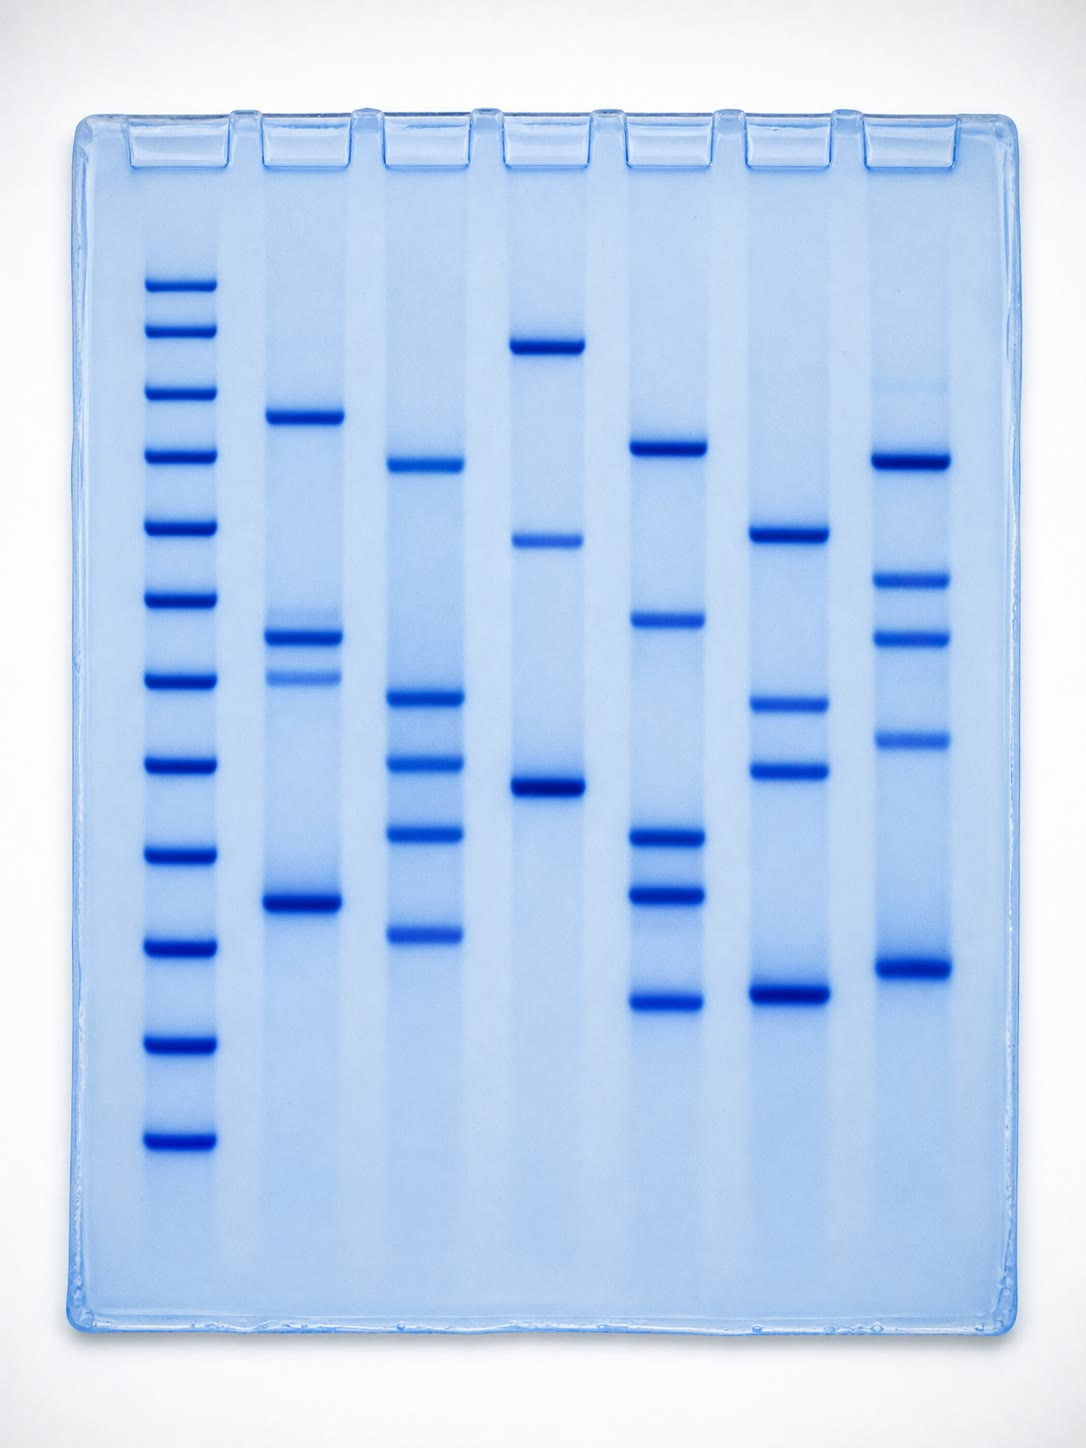
\includegraphics[width=0.36\linewidth]{images/book3/ai/b3-12-protein-gel.jpg}

{\small 染色后的 SDS--聚丙烯酰胺凝胶。每条泳道为一个样品，
各条带为一种大小的\omterm{def:b1:proteins:peptide}{蛋白质}；最左侧泳道为已知
质量的标准梯。小\omterm{def:b1:proteins:peptide}{蛋白质}迁移得更远。}
\end{omfigure}

\begin{example}[读凝胶]\label{ex:b1:proteins:gel}
粗提物的电泳图上有数十条带；经亲和层析后
仅剩一条带，位于 \qty{33}{kDa} 标志物的位置。若
不加 SDS、也不加还原剂进行电泳，同一\omterm{def:b1:proteins:peptide}{蛋白质}迁移为一个
\qty{66}{kDa} 的分子：它是两条相同的链，由一个
\omterm{def:b1:proteins:tertiary}{二硫键}相连的二聚体，还原剂可打断该键，去污剂则
使两条链分开。两块凝胶、一条推理，\omterm{def:b1:proteins:tertiary}{四级结构}
即已可知。
\end{example}

\section{练习}

\begin{exercise}[$\star$]\label{exo:b1:proteins:1}
画出或描述 \omterm{def:b1:water-small-molecules:ph}{pH} 7 时\omterm{def:b1:proteins:aminoacid}{氨基酸}的一般结构，并
按\omterm{def:b1:proteins:aminoacid}{侧链}对 Leu、Ser、Lys、Glu 和 Phe 进行分类。
\end{exercise}

\begin{exercise}[$\star$]\label{exo:b1:proteins:2}
定义\omterm{def:b1:proteins:peptide}{蛋白质}结构的四个层次，并说明维持
每一层次的化学键。
\end{exercise}

\begin{exercise}[$\star$]\label{exo:b1:proteins:3}
某\omterm{def:b1:proteins:peptide}{蛋白质}含 \qty{450}{} 个残基。估算其质量。若它
为单个 $\alpha$ 螺旋，其长度为多少？单条 $\beta$ 链呢？
\end{exercise}

\begin{exercise}[$\star$]\label{exo:b1:proteins:4}
由氧结合图读出血红蛋白在
\qty{13.3}{kPa} 与 \qty{5.3}{kPa} 下的饱和度，并求输送的比例。
\end{exercise}

\begin{exercise}[$\star\star$]\label{exo:b1:proteins:5}
计算肽 Lys--Gly--Asp--Ala 在 \omterm{def:b1:water-small-molecules:ph}{pH} 7、
\omterm{def:b1:water-small-molecules:ph}{pH} 2 和 \omterm{def:b1:water-small-molecules:ph}{pH} 12 时的净电荷，利用本章的 p$K_a$ 值，并估算
其\omterm{prop:b1:proteins:ionisation}{等电点}。
\end{exercise}

\begin{exercise}[$\star\star$]\label{exo:b1:proteins:6}
解释脯氨酸为何很少出现在 $\alpha$ 螺旋内部，以及为何
甘氨酸却常见于紧密转角处，并从主链的几何结构加以说明。
\end{exercise}

\begin{exercise}[$\star\star$]\label{exo:b1:proteins:7}
在安芬森的实验中，随机重新氧化能得到天然的
四对\omterm{def:b1:proteins:tertiary}{二硫键}的比例是多少？（计算八个半胱氨酸
配对的方式数。）实际恢复的全部活性
证明了什么？
\end{exercise}

\begin{exercise}[$\star\star$]\label{exo:b1:proteins:8}
利用\omterm{def:b1:proteins:allostery}{希尔方程}，取 $n = 2.8$ 与 $P_{50} = \qty{3.5}{kPa}$，
求 $Y$ 在 \qty{2}{kPa}、\qty{3.5}{kPa} 和 \qty{8}{kPa} 时的值。
再取 $n = 1$ 重复计算。哪种\omterm{def:b1:proteins:peptide}{蛋白质}在 \qty{8}{} 与
\qty{2}{kPa} 之间输送的氧更多？
\end{exercise}

\begin{exercise}[$\star\star$]\label{exo:b1:proteins:9}
某\omterm{def:b1:proteins:peptide}{蛋白质}在 SDS 凝胶上呈单一条带（\qty{50}{kDa}），
经凝胶过滤柱洗脱时位于 \qty{200}{kDa} 处。
写出其\omterm{def:b1:proteins:tertiary}{四级结构}，并说明如何检验
亚基之间是否存在\omterm{def:b1:proteins:tertiary}{二硫键}。
\end{exercise}

\begin{exercise}[$\star\star\star$]\label{exo:b1:proteins:10}
镰状\omterm{def:b1:cell-unit-of-life:cell}{细胞}血红蛋白的 $\beta$ 链第 6 位（表面）
处以缬氨酸代替了谷氨酸。试从两种\omterm{def:b1:proteins:aminoacid}{侧链}的化学性质出发，
解释突变蛋白为何在脱氧时发生聚合，
以及病变为何出现在\omterm{def:b1:body-plans-tissues:tissue}{组织}中，而不是在
肺部。
\end{exercise}

\begin{exercise}[$\star\star\star$]\label{exo:b1:proteins:11}
某折叠结构的稳定性仅为 \qty{40}{kJ/mol}。求平衡时
在 \qty{37}{\celsius} 下未展开分子所占的比例（$K = e^{-\Delta G/RT}$），
以及若 $\Delta G$ 降至 \qty{10}{kJ/mol}，则在 \qty{45}{\celsius} 下的比例。
为何这样不高的稳定性对\omterm{def:b1:cell-unit-of-life:cell}{细胞}有利？
\end{exercise}

\begin{exercise}[$\star\star\star$]\label{exo:b1:proteins:12}
“\omterm{def:b1:proteins:peptide}{蛋白质}是折叠成某一形状的序列，而形状即是
功能。”请结合安芬森、\omterm{prop:b1:proteins:denaturation}{分子伴侣}、镰状\omterm{def:b1:cell-unit-of-life:cell}{细胞}病与\omterm{def:b1:proteins:allostery}{别构作用}，写一段话讨论：
该句在哪些情形下成立，以及\omterm{def:b1:cell-unit-of-life:cell}{细胞}
必须在何处进行干预。
\end{exercise}

\section{问题：工作中的血红蛋白}

\begin{problem}[{周末问题——氧气从肺运输至
肌肉，分别在静息、短跑、高山与出生前的情形下，最后落在
每升血液输送的氧气量}]
\label{pb:b1:proteins:1}
血液中含有 \qty{150}{g/L} 的血红蛋白；\qty{1}{g} 可结合
\qty{1.34}{mL} 的 $\mathrm{O_2}$。血红蛋白遵循\omterm{def:b1:proteins:allostery}{希尔方程}，
在 \omterm{def:b1:water-small-molecules:ph}{pH} 7.4 时，$n = 2.8$，$P_{50} = \qty{3.5}{kPa}$；肌红蛋白的
$n = 1$，$P_{50} = \qty{0.37}{kPa}$。$\mathrm{O_2}$ 的分压为：
海平面时肺中为 \qty{13.3}{kPa}，
静息\omterm{def:b1:body-plans-tissues:tissue}{组织}中为 \qty{5.3}{kPa}。取 $2.8\ln 3.5 = 3.51$，
$2.8\ln 5.3 = 4.67$, $2.8\ln 13.3 = 7.25$, $2.8\ln 2.7 = 2.78$,
$2.8\ln 4.5 = 4.21$, $2.8\ln 7 = 5.45$, $2.8\ln 4 = 3.88$,
$2.8\ln 2.6 = 2.68$.

\medskip
\noindent\textbf{第一部分——静息时。}
\begin{enumerate}
  \item 求每升血液的氧容量。
  \item 求 $P^{2.8}$，其中 $P = 3.5$、$5.3$ 和 $13.3$ kPa（
        即 $e^{2.8\ln P}$）。
  \item 求血红蛋白在肺部和\omterm{def:b1:body-plans-tissues:tissue}{组织}中的饱和度
        $Y$。
  \item 求所输送负荷的比例，以及每升血液输送的氧量，
        以毫升为单位。
  \item 静息的人每分钟消耗 \qty{250}{mL} 的 $\mathrm{O_2}$，
        该输送量需要多大的心输出量？
  \item 求肌红蛋白在相同两个压强下的饱和度，
        以及若其替代血红蛋白时每升血液能输送的氧量，
        并作出结论。
  \item 用一句话说明\omterm{def:b1:proteins:allostery}{协同性}带来了什么好处。
\end{enumerate}

\medskip
\noindent\textbf{第二部分——短跑。}
在短跑时的肌肉中，\omterm{def:b1:water-small-molecules:ph}{pH} 降至 7.2，局部
$\mathrm{O_2}$ 压强降至 \qty{2.7}{kPa}；玻尔效应使该处的 $P_{50}$ 升至
\qty{4.5}{kPa}。
\begin{enumerate}[resume]
  \item 求 \qty{2.7}{kPa} 时的 $Y$，取 $P_{50} = \qty{3.5}{kPa}$
        （无玻尔效应）。
  \item 求 \qty{2.7}{kPa} 时的 $Y$，取 $P_{50} = \qty{4.5}{kPa}$。
  \item 求两种情形下每升血液输送的氧量
        （肺中载氧量保持不变），以及玻尔效应所带来的
        增益。
  \item 该肌肉中的肌红蛋白处于 $P = \qty{2.7}{kPa}$。其
        饱和度为多少？若收缩期间压强降至
        \qty{0.5}{kPa}，它会发生什么变化？
  \item 解释玻尔效应为何属于\omterm{def:b1:proteins:allostery}{别构作用}，以及质子
        在何处发挥作用。
\end{enumerate}

\medskip
\noindent\textbf{第三部分——高山。}
在海拔 \qty{4000}{m} 处，肺中的 $\mathrm{O_2}$ 压强为 \qty{7}{kPa}。
数日之内，红\omterm{def:b1:cell-unit-of-life:cell}{细胞}提高其 BPG 含量，使 $P_{50}$ 升至
\qty{4.0}{kPa}；数周之内，骨髓将血红蛋白提高至
\qty{180}{g/L}。
\begin{enumerate}[resume]
  \item 求 \qty{7}{kPa} 时肺中的饱和度，取
        $P_{50} = \qty{3.5}{kPa}$，以及每升血液的输送量（\omterm{def:b1:body-plans-tissues:tissue}{组织}中
        压强为 \qty{5.3}{kPa}），并与海平面情况作比较。
  \item 求肺与\omterm{def:b1:body-plans-tissues:tissue}{组织}中的饱和度，取
        $P_{50} = \qty{4.0}{kPa}$，以及输送量。
  \item 解释为何降低亲和力有利，尽管它会降低
        肺中的载氧量。
  \item 求取 $P_{50} = \qty{4.0}{kPa}$ 且血红蛋白为
        \qty{180}{g/L} 时每升血液的输送量。
  \item 若亲和力进一步降低（$P_{50} = \qty{6}{kPa}$），
        在 \qty{7}{kPa} 时是否更有帮助？求两个饱和度并作出判断。
\end{enumerate}

\medskip
\noindent\textbf{第四部分——出生前。}
胎儿血红蛋白 $P_{50} = \qty{2.6}{kPa}$；在胎盘中，
母体与胎儿两侧的 $\mathrm{O_2}$ 压强均为 \qty{4}{kPa}。
\begin{enumerate}[resume]
  \item 求母体血红蛋白在 \qty{4}{kPa} 下的饱和度。
  \item 求胎儿血红蛋白在 \qty{4}{kPa} 下的饱和度。
  \item 解释尽管两侧压强相同，氧气如何从母体
        转移至胎儿。
  \item 胎儿血红蛋白以 $\gamma$ 链代替 $\beta$ 链，其
        与 BPG 的结合较弱。解释这如何使 $P_{50}$ 更低。
  \item 出生时，胎儿血液须在\omterm{def:b1:body-plans-tissues:tissue}{组织}中于
        \qty{5.3}{kPa} 下卸载。求胎儿血液每升从肺部
        （\qty{13.3}{kPa}）所输送的量，并说明出生后头几个月
        转换为成人血红蛋白为何有利。
  \item 一次突变使成人的 $P_{50}$ 升至 \qty{5}{kPa}。预测
        此人在海平面的动脉血饱和度，以及
        对输送量的影响。
  \item 解释一个 $P_{50} = \qty{3.5}{kPa}$ 且无\omterm{def:b1:proteins:allostery}{协同性}的载体，
        （$n = 1$）为何是较差的载氧体，求其
        输送量。
  \item 给出结论：每升血液输送的氧量，
        静息与短跑肌肉中的氧输送量，以及使两者产生差异的
        血红蛋白的两种性质。
\end{enumerate}
\end{problem}
